\chapter{Related work}

In this chapter, we present prior research related to IoT security. We present the previous approaches and discuss the differences between our approach and existing work.

In addition to security, we also review previous research related to IoT \textit{anonymity}. Several papers attempt to use the Tor network in concert with IoT systems to achieve anonymity, but the problem has not been studied in great depth, as we discuss below. 

\section{IoT security and privacy}

IoT security and privacy has been studied widely. Alrawi \textit{et al.} \cite{alrawi2019sok} provide an overview of security study challenges in modern IoT systems. In their work, they propose a modeling methodology to study home-based IoT devices and evaluate their security posture based on component analysis. Lin \textit{et al.} \cite{lin2016iot} survey existing solutions for enhancing IoT security and identify key feature requirements for trusted smart home systems. They point out two key technologies, support for system auto-configuration and automatic update of system firmware. 


In terms of privacy-preserving structures for IoT systems, researchers have proposed many protocols covering different aspects of privacy. Song \textit{et al.} \cite{song2017privacy} design a privacy-preserving communication protocol for IoT applications. Their protocol enables IoT appliances and sensors to communicate with a central controller securely and ensures data integrity and authentication by incorporating Message Authentication Codes (MACs, which protects messages' integrity and authenticity by allowing verifiers to detect any changes to the message content) to the data transmission. While we are not focused on protecting the veracity of IoT measurements in this thesis and would like a decentralized structure for anonymity, the incorporation of MACs might be applicable.


Fabian \textit{et al.} \cite{fabian2014privacy} introduce a privacy-preserving P2P data infrastructure for IoT devices based on the Octopus distributed hash table \cite{wang2012octopus} and measured the efficiency of their infrastructure (latency) using simulated networks. While our design does not cover storage issues (the data are only stored locally and discarded immediately after served to the user), it is possible to extend our design by adapting their solution.

Apthorpe \textit{et al.} \cite{apthorpe2017smart} review privacy vulnerabilities in encrypted IoT traffic of four commercial IoT services. In addition, they develop a strategy to infer consumer behavior from rates of IoT traffic, which enables a passive network observer to retrieve information even when the traffic is encrypted. In this thesis, we use two strategies to avoid such traffic analysis. Firstly, when possible, we use Tor to obfuscate the network location and traffic of IoT devices. Secondly, we cover the traffic to make traffic analysis more difficult.

There are also work focusing on the security of pairing devices. Au \cite{au2012pscout} perform an analysis of the permission of Android, and propose a tool to analyze the security issues of permission specification. Egele \cite{egele2013empirical} develop program analysis techniques to automatically check programs on cryptographic misuse (whether the cryptographic APIs provides typical cryptographic notions of security, e.g. IND-CPA). In Section \ref{sec:case_study} of this thesis, we implement an example Android app, and strictly follow the correct usage of permissions and cryptographic functions to prevent security issues.



\section{Anonymity and IoT}

Moving towards anonymous communication for IoT systems, there have been approaches utilizing onion networks. Hiller \textit{et al.} \cite{hiller2019tailoring} propose a mechanism to tailor onion routing to IoT by bridging the protocol incompatibilities and securely offloading expensive computations to an external server owned by the IoT device owner. Their work focuses on solving problems of incompatible protocols and constrained resources. While our approach proposes a framework for privacy-preserving IoT functionality, Hiller \textit{et al.}'s optimization is also applicable to our approach to provide a more generalized design for privacy-preserving IoT systems.

Hoang \textit{et al.} \cite{hoang2015tor} discuss the challenges and benefits of using the Tor network to secure smart home appliances. They list several  vulnerabilities that IoT users face and show how Tor-based communication can help users protect their privacy. This thesis presents a concrete privacy-preserving design for generalized IoT devices and implementation for a specific type of IoT device (an Internet-enabled video doorbell).

Focusing on enhanced security communication for IoT addressing and connectivity, Baumann \textit{et al.} \cite{baumann2018utilising} discuss how utilizing Tor benefits in environments behind firewalls, proxies and NAT. They propose a prototype implementation of an Internet-enabled 3D printer using a RaspberryPi as the hardware. Our approach provides a more general framework for IoT security and privacy, and our use case covers a different category of IoT device.

\section{Background on Tor}
\label{sec:torbackground}
The Tor network, which was developed in the 1990s and deployed in 2002, is an overlay protocol to route traffic through multiple servers and encrypt it each step of the way (\cite{torproject}, \cite{chaabane2010digging}). By directing internet traffic through the onion network, which consists of several thousand volunteer overlays, Tor conceals users' locations and usage from adversaries.

Tor allows the creation of \textit{Hidden Services}, which conceal the network locations of Internet services. Such services are only reachable within the onion network by users running the Tor client. Hidden services are identified by \textit{.onion} addresses.

Several features of Tor make it attractive for privacy-preserving IoT communications. Because the nature of Tor requires all peers to be connected, Tor maintains the connections after they are initiated to build the circuits. As a side-effect, all peers can receive data regardless of whether they are behind a firewall or NAT. \textit{Fig. \ref{fig:natpiercing}} shows the network structure of a IoT system adopting the onion network. In such a system, both the IoT device and the end-user device keeps an outgoing TCP connection with onion relays, and thus does not require a static IP address.

These features, including providing NAT piercing and prevention of DoS attacks, are essential for home IoT devices (as home IoT devices are usually located in typical home networks, which tend to be behind NAT). Furthermore, the system of Tor is actively maintained and improved.

\begin{figure}
	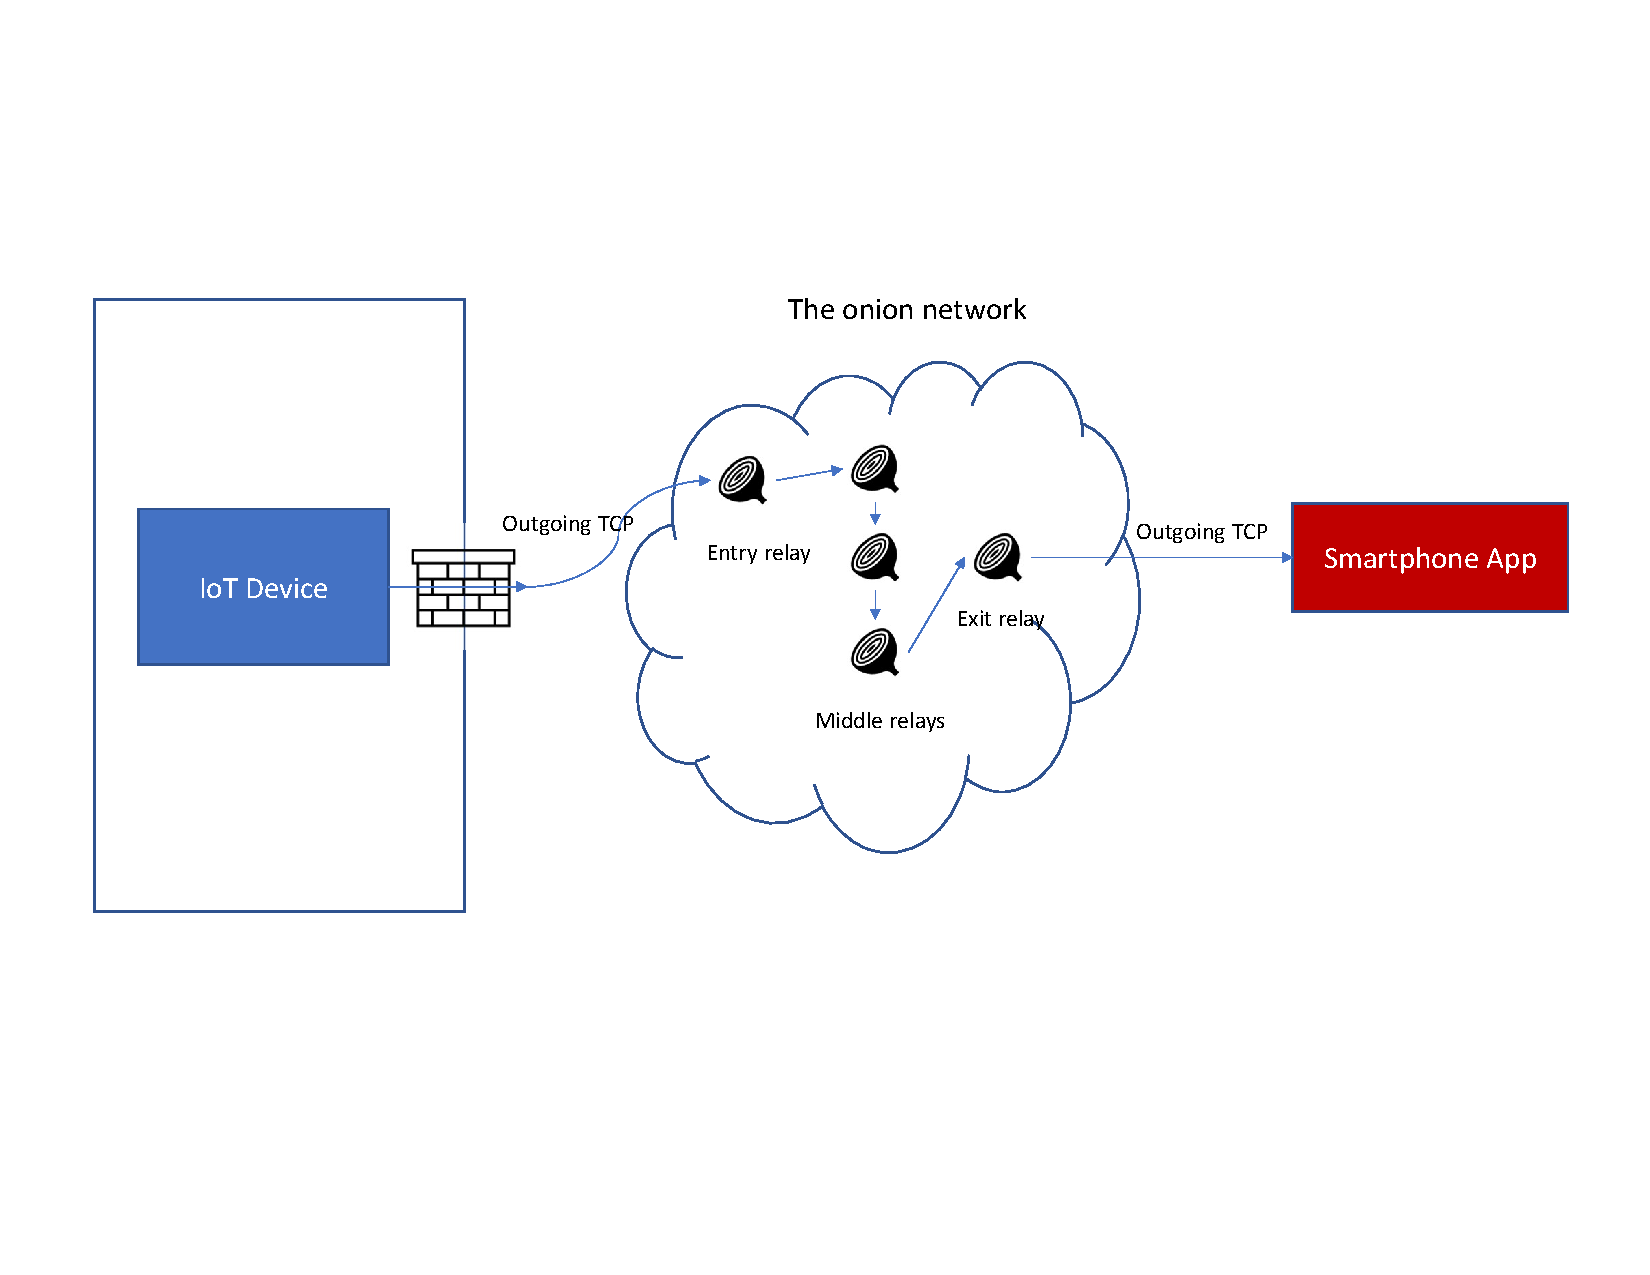
\includegraphics[width=\linewidth]{natpiercing.pdf}
	\caption{Network Structure of onion-IoT}
	\label{fig:natpiercing}
\end{figure}